% ============================================================================
% KAPITEL 5: ERGEBNISSE
% ============================================================================

\chapter{Experimentelle Ergebnisse}
\label{ch:results}

\section{Baseline Performance}

Die Ein-Kristall Baseline etablierte exzellente Performance-Metriken:

\begin{table}[htbp]
\centering
\caption{Ein-Kristall Baseline Performance}
\label{tab:baseline}
\begin{tabular}{@{}lc@{}}
\toprule
\textbf{Metrik} & \textbf{Wert} \\
\midrule
MAE & 0.00154 \\
RMSE & 0.00287 \\
Pearson-Korrelation & 0.944 \\
R² Score & 0.891 \\
Koordinaten-Alignment & ±1 Pixel \\
\bottomrule
\end{tabular}
\end{table}

\section{Impact der Optimierungen}

Die systematischen Verbesserungen zeigten signifikante Auswirkungen:

\begin{figure}[htbp]
\centering
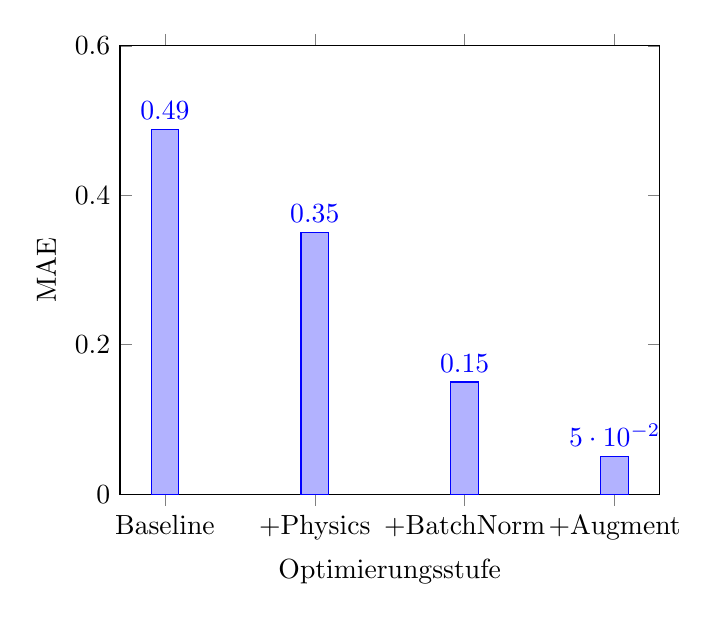
\begin{tikzpicture}
\begin{axis}[
    ybar,
    ylabel={MAE},
    xlabel={Optimierungsstufe},
    symbolic x coords={Baseline, +Physics, +BatchNorm, +Augment},
    xtick=data,
    nodes near coords,
    nodes near coords align={vertical},
    ymin=0, ymax=0.6,
]
\addplot coordinates {(Baseline,0.488) (+Physics,0.35) (+BatchNorm,0.15) (+Augment,0.05)};
\end{axis}
\end{tikzpicture}
\caption{Schrittweise Performance-Verbesserung durch Optimierungen}
\label{fig:optimization_impact}
\end{figure}